\section{问题二的模型与求解}

\subsection{日前新能源功率预测}

\subsubsection{严格因果的验证方案}

问题二需要在目标日开始前给出全天 $144$ 个时段的新能源发电功率。记第 $d$ 个运营日第
$t$ 个时段的实测功率为 $P_{d,t}$，预测值为 $\widehat{P}_{d,t}$。为使预测误差能够直接服务于
后续调度，本节以完整运营日为滚动预测单位，所有模型使用相同的验证起点和评价时段。

模型选择仅使用 2025 年 1 月 18 日至 1 月 31 日的 $14$ 个滚动预测日。对每个预测日，训练样本
的目标结束时刻与标准化统计量的最晚时刻均严格早于该日首个目标时刻。候选模型及超参数按照
验证期整体 RMSE 从小到大排序，若 RMSE 相同，则以 MAE 较小者优先。模型一经选定，其结构、
参数、标准化统计量及融合权重在 2025 年 2 月 1 日至 12 月 31 日的正式评价期内保持不变；新到达
的实测数据仅用于构造历史输入，不参与参数更新。因此，正式期结果不反向参与模型或超参数选择。

\subsubsection{候选模型}

为检验复杂模型相对于周期规律的实际增益，本文在同一因果协议下比较以下八类方法：

\begin{enumerate}
  \item \textbf{昨日同刻（Yesterday）}：$\widehat{P}_{d,t}=P_{d-1,t}$；
  \item \textbf{上周同刻（Last Week）}：$\widehat{P}_{d,t}=P_{d-7,t}$；
  \item \textbf{近 7 日同刻均值}：
  $\widehat{P}_{d,t}=\frac{1}{7}\sum_{j=1}^{7}P_{d-j,t}$；
  \item \textbf{相位模型（Phase）}：以权重 $\alpha$ 融合昨日同刻和上周同刻预测，
  $\widehat{P}^{\mathrm{ph}}_{d,t}=\alpha P_{d-1,t}+(1-\alpha)P_{d-7,t}$，其中
  $\alpha\in\{0,0.05,\ldots,1\}$ 仅由一月验证期确定；
  \item \textbf{奇异谱分析（SSA）}：对预测日前的历史序列作均值中心化和 Hankel 嵌入，保留
  验证期选定的低秩信号子空间，并通过递推关系生成未来 $144$ 个时段；
  \item \textbf{DLinear}：先以移动平均将历史序列分解为趋势项与余项，再分别进行线性投影并
  求和。输入窗、移动平均核及因果标准化方式均只在一月确定；
  \item \textbf{结构--残差混合（StructuralResidualHybrid）}：以低秩解析结构分量作为教师，
  使用轻量残差网络修正其未能解释的短期变化，最终仅施加新能源功率非负约束；
  \item \textbf{相位--结构融合（PhaseStructuralFusion）}：以固定权重融合相位模型与结构--残差
  混合模型，融合权重在一月验证期内按 $0.05$ 的步长选择。
\end{enumerate}

上述比较不使用附件 3 的官方预报，也不在正式评价期执行在线重训练。相位模型选得
$\alpha=0.55$；DLinear 在其候选族中选得 7 日输入窗、73 点移动平均核和因果 $z$-score；
结构--残差混合模型选得 7 日输入窗及 144 行 Hankel 矩阵。相位--结构融合的相位权重为
$1.00$，说明一月验证未支持在最终点预测中加入结构修正分量。

\subsubsection{预测结果与模型选择}

表~\ref{tab:q2-forecast-comparison} 汇总了统一验证期和正式评价期的结果。近 7 日同刻均值在一月
验证期取得最低 RMSE，为 $213.551\ \mathrm{kW}$，相应 MAE 为 $101.382\ \mathrm{kW}$，因此按预先
规定的规则被选为新能源发电功率的正式预测模型。该模型在 2 月至 12 月冻结评价期的 RMSE 为
$303.858\ \mathrm{kW}$，MAE 为 $153.400\ \mathrm{kW}$。图~\ref{fig:q2-final-forecast-comparison}
将选型依据与正式期误差分列展示，其中正式期结果仅用于检验泛化性能，不参与模型选择。

\begin{table}[H]
  \centering
  \caption{新能源发电功率候选模型的统一因果比较}
  \label{tab:q2-forecast-comparison}
  \small
  \setlength{\tabcolsep}{4pt}
  \begin{tabularx}{\textwidth}{>{\raggedright\arraybackslash}Xrrrrc}
    \toprule
    \multirow{2}{*}{模型} & \multicolumn{2}{c}{一月验证期} &
    \multicolumn{2}{c}{2--12 月正式期} & \multirow{2}{*}{入选} \\
    \cmidrule(lr){2-3}\cmidrule(lr){4-5}
     & MAE & RMSE & MAE & RMSE & \\
    \midrule
    昨日同刻 & 125.244 & 272.937 & 185.346 & 375.175 &  \\
    上周同刻 & 143.422 & 291.266 & 214.688 & 419.948 &  \\
    近 7 日同刻均值 & 101.382 & 213.551 & 153.400 & 303.858 & $\checkmark$ \\
    相位模型 & 116.045 & 242.959 & 170.571 & 341.373 &  \\
    SSA & 219.383 & 334.147 & 260.834 & 393.833 &  \\
    DLinear & 151.795 & 261.481 & 423.397 & 692.692 &  \\
    结构--残差混合 & 872.672 & 1397.551 & 1400.663 & 1993.198 &  \\
    相位--结构融合 & 116.045 & 242.959 & 170.571 & 341.373 &  \\
    \bottomrule
  \end{tabularx}
  \vspace{2pt}
  \begin{minipage}{0.96\textwidth}
    \footnotesize 注：误差单位均为 kW；表中数值由
    \texttt{forecast\_model\_final\_comparison.csv} 生成。入选标记仅依据一月验证期。
  \end{minipage}
\end{table}

\begin{figure}[H]
  \centering
  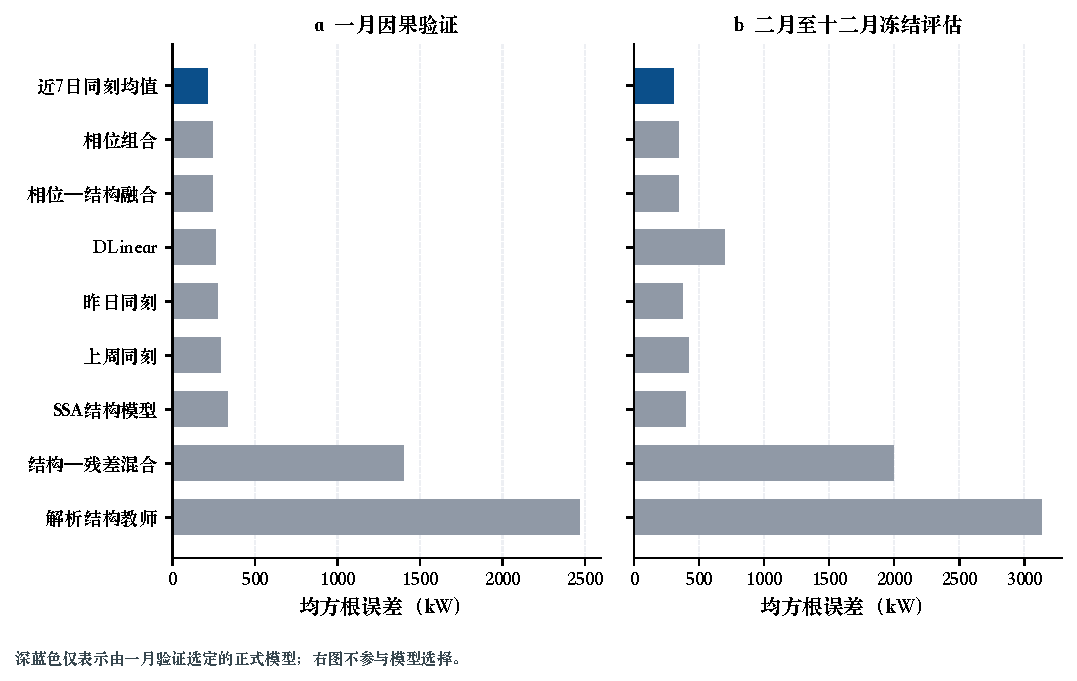
\includegraphics[width=0.94\textwidth]{../results/problem2/figures/fig_p2_final_forecast_comparison.pdf}
  \caption{候选模型在一月统一验证期与 2--12 月冻结评价期的 RMSE。深蓝色表示仅依据一月
  验证选定的正式模型；右图不参与模型选择。}
  \label{fig:q2-final-forecast-comparison}
\end{figure}

低秩奇异谱的能量集中表明新能源序列具有明显的低维结构，但结构可压缩性并不等价于多步预测
误差最小。统一因果比较显示，增加分解、学习和融合复杂度未带来足以改变选择的验证期增益，故
本文保留更简洁且稳定的近 7 日同刻均值。由于正式预测器未发生变化，既有点预测文件、配对整日
残差场景及其时间泄露审计结果均保持不变。本节至此仅完成预测模型选定，不涉及后续调度优化。
